140. \begin{figure}[ht!]
\center{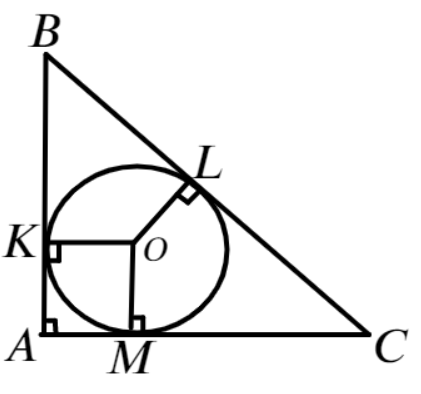
\includegraphics[scale=0.35]{g8-71.png}}
\end{figure}\\
Проведём радиусы к точкам касания. Так как отрезки касательных, проведённых из одной точки, равны, имеем $AK=AM,\ BK=BL,\ CL=CM.$ Так как $AKOM$ прямоугольник и $AK=AM,$ он является квадратом и радиус окружности тоже равен $AK.$ Пусть $AK=AM=x,$ тогда $AB=x+5,\ AC=x+12,\ BC=5+12=17$ и по теореме Пифагора для треугольника $ABC$ получаем $(x+5)^2+(x+12)^2=17^2,\ x^2+10x+25+x^2+24x+144=289,\ 2x^2+34x-120=0,\ x^2+17x-60=0,\ x=3.$ Тогда катеты равны $3+5=8$ и $3+12=15.$\\
